\chapter{Interview Guide}
\label{app:interview-guide}

This appendix records the scenario-based moderator script used in the evaluation interviews. The wording follows the version spoken in sessions (including the consent statement and scenario prompts). Each numbered question lists the \textbf{linked research questions} (Main~RQ and RQ1--RQ5) taken from the analysis mapping used alongside the guide: RQ1 addresses current platform limitations; RQ2 expectations and post-sharing concerns; RQ3 clarity of the interface and permission model; RQ4 fairness and social implications; RQ5 trust, safety, control, and realism of revocation. The main research question is stated in Chapter~1.

\section*{Research question key}
\begin{description}[style=nextline,leftmargin=0.8cm]
  \item[Main~RQ] Overall contribution of the proposed design.
  \item[RQ1] Limitations of current platforms for controlling shared photos.
  \item[RQ2] User expectations, practices, and concerns about post-sharing control.
  \item[RQ3] Clarity and understandability of the interface and permission model.
  \item[RQ4] Social implications for stakeholders.
  \item[RQ5] Trust, safety, perceived control, and realism of revocation.
\end{description}

\section{Section 0: Mandatory consent statement}
\textit{Say verbatim:}

\begin{quote}\small\sloppy
``Before we begin, I'd like to confirm your consent to participate in this interview. This interview is part of my research on how messaging platforms might support consent revocation for shared photos. The purpose of this interview is to understand your views and reactions to a design concept. During the interview, I will show you example screens from a prototype. I am not testing you --- I am testing the design. There are no right or wrong answers, and honest reactions are very helpful. Some questions are about privacy, control, and what happens to photos after they are shared. You can skip any question or stop the interview at any time. With your permission, I would like to audio-record this interview so I can analyse the responses later. The recording will only be used for this project, and your responses will be anonymised. You can choose to stop the recording or withdraw from the interview at any time. If you're happy to proceed, could you please state your full name and age, and confirm that you agree to be interviewed and recorded?''
\end{quote}

\section{Section 1: Warm-up and current photo-sharing behaviour}


\begin{enumerate}
  \item \textbf{Can you tell me a bit about how you usually share photos on apps like WhatsApp?}\\
  \textit{Linked:} RQ2.\\
  \textit{Probes optional:} private vs group chats; casual vs personal photos; frequency.

  \item \textbf{When you send a photo to someone, do you usually think about what might happen to it afterwards? If yes, what kinds of concerns or challenges come to mind?}\\
  \textit{Linked:} RQ2.\\
  \textit{Probes optional:} saving, forwarding, screenshots, long-term retention; active vs incidental thought.

  \item \textbf{Have you ever wanted more control over a photo after you had already sent it?}\\
  \textit{Linked:} RQ1; RQ2.\\
  \textit{Probes optional:} type of control wished for; whether the app helped.

  \item \textbf{What do you think current apps do well or badly when it comes to controlling shared photos?}\\
  \textit{Linked:} RQ1.
\end{enumerate}


\section{Section 2: Scenario 1 --- Before sending a photo}
\textit{Show:} photo composer / permission setup (view once, forwarding, download, co-subject, time limit; note on screenshots and saves).


\begin{enumerate}[resume]
  \item \textbf{What do you think is happening on this screen?}\\
  \textit{Linked:} RQ3.\\
  \textit{Probes optional:} purpose of controls; what the sender decides.

  \item \textbf{What do you think each of these settings means?}\\
  \textit{Linked:} RQ3.\\
  \textit{Probes optional:} view once; forwarding disabled; download disabled; time limit; co-subject in photo.

  \item \textbf{Which of these options feel useful to you, and which feel unnecessary or unclear?}\\
  \textit{Linked:} RQ2; RQ3.\\
  \textit{Probes optional:} realistic pre-send use; effort; missing options.

  \item \textbf{There is also a warning here saying that screenshots and saves cannot be undone. How do you feel about that?}\\
  \textit{Linked:} RQ3; RQ5.\\
  \textit{Probes optional:} honesty vs usefulness; whether the warning is wanted.
\end{enumerate}

\textit{Moderator note:} Only explain controls if the participant is completely stuck; prior interpretation is the primary data.

\section{Section 3: Scenario 2 --- Changing permissions after sending}
\textit{Show:} sent photo with photo menu (revoke/restore, forwarding, download, time limit).


\begin{enumerate}[resume]
  \item \textbf{Looking at this screen, what do you think the sender is able to do now?}\\
  \textit{Linked:} RQ3.\\
  \textit{Probes optional:} what is changeable after send; comparison to deleting a message; revoke vs permission change.

  \item \textbf{What would you expect to happen if the sender revokes access here?}\\
  \textit{Linked:} RQ3; RQ5.\\
  \textit{Probes optional:} visibility; recipient notification; offline copies; if already seen.

  \item \textbf{How understandable does this post-send control feel to you?}\\
  \textit{Linked:} RQ3.\\
  \textit{Probes optional:} clarity of change; menu affordances; discoverability.

  \item \textbf{Would this kind of feature make you feel more in control after sending a photo? Why or why not?}\\
  \textit{Linked:} RQ5.\\
  \textit{Probes optional:} trust; anxiety; realistic use.
\end{enumerate}

\textit{Moderator note:} Keep focus on clarity, expectations, realism, and perceived control rather than implementation detail.

\section{Section 4: Scenario 3 --- Recipient view, request access, and fairness}
\textit{Show:} recipient-side revoked placeholder (screenshots / prior viewing note).


\begin{enumerate}[resume]
  \item \textbf{What do you think this screen is telling the recipient?}\\
  \textit{Linked:} RQ3; RQ4.\\
  \textit{Probes optional:} clarity of change; sufficiency of explanation.

  \item \textbf{How would you feel if you were the recipient in this situation?}\\
  \textit{Linked:} RQ4; RQ5.\\
  \textit{Probes optional:} reasonable vs awkward; fairness tone.

  \item \textbf{What do you think about the idea that the recipient can request access again?}\\
  \textit{Linked:} RQ4.\\
  \textit{Probes optional:} comfort as sender or recipient; balance.

  \item \textbf{Does this feel fair to both people, or more fair to one side than the other?}\\
  \textit{Linked:} RQ4.\\
  \textit{Probes optional:} sender power; explanation; objection rights.

  \item \textbf{What do you think about the wording used here?}\\
  \textit{Linked:} RQ4.\\
  \textit{Probes optional:} neutrality vs blame.
\end{enumerate}

\textit{Moderator note:} Do not defend the revoked state; negative reactions are informative.

\section{Section 5: Scenario 4 --- Forwarding and residual concerns}
\textit{Show:} forwarding behaviour and secondary recipient where relevant; request-access flow and sender accept/reject if shown.


\begin{enumerate}[resume]
  \item \textbf{What do you think this forwarding feature is trying to do?}\\
  \textit{Linked:} RQ3.\\
  \textit{Probes optional:} blocked vs allowed forwarding; sender rules after forward.

  \item \textbf{How do you feel about the idea that the sender's rules continue even after the photo is forwarded?}\\
  \textit{Linked:} RQ3; RQ5.\\
  \textit{Probes optional:} usefulness; realism; over-control.

  \item \textbf{Even with these features, what concerns would still remain for you?}\\
  \textit{Linked:} RQ1; RQ2; RQ5.\\
  \textit{Probes optional:} screenshots; prior downloads; residual value of imperfect control.
\end{enumerate}

\section{Section 6: Scenario 5 --- Co-subject request for revocation}
\textit{Show:} co-subject notification and request flow; sender accept/reject.


\begin{enumerate}[resume]
  \item \textbf{What do you think about that idea?}\\
  \textit{Linked:} RQ4; RQ5.\\
  \textit{Probes optional:} fairness; invasiveness; complexity.

  \item \textbf{For this kind of scenario where the photo includes the sender and other co-subjects, who do you think should have the strongest control in that situation: the sender, the person in the photo, both equally, or someone else?}\\
  \textit{Linked:} RQ4.

  \item \textbf{How realistic does this feel in a real messaging app?}\\
  \textit{Linked:} RQ5.
\end{enumerate}

\textit{Moderator note:} Use only if time allows or if co-subject control is a session focus.

\section{Section 7: Wrap-up and final reflections}


\begin{enumerate}[resume]
  \setcounter{enumi}{24}
  \item \textbf{Would this make you feel more in control when sharing personal photos? Why or why not?}\\
  \textit{Linked:} RQ5.

  \item \textbf{Would it make you trust the platform more, less, or no differently?}\\
  \textit{Linked:} RQ5.

  \item \textbf{What part felt most clear or useful?}\\
  \textit{Linked:} RQ3; RQ5.

  \item \textbf{What part felt most confusing, unrealistic, or uncomfortable?}\\
  \textit{Linked:} RQ1; RQ3; RQ5.

  \item \textbf{From 1 to 5, how clear do you think everything feels?}\\
  \textit{Linked:} RQ3.
\end{enumerate}

\newpage
\section{Interview scenario slides (stimulus material)}
\label{app:interview-scenario-slides}

\noindent
This section reproduces the slide deck \emph{Consent Revocation Interview Scenarios}. The screenshots embedded in these slides were taken from the \textbf{first round} of the prototype implementation, before later visual or interaction refinements and they are preserved here to document the materials participants actually saw.

\begin{center}
  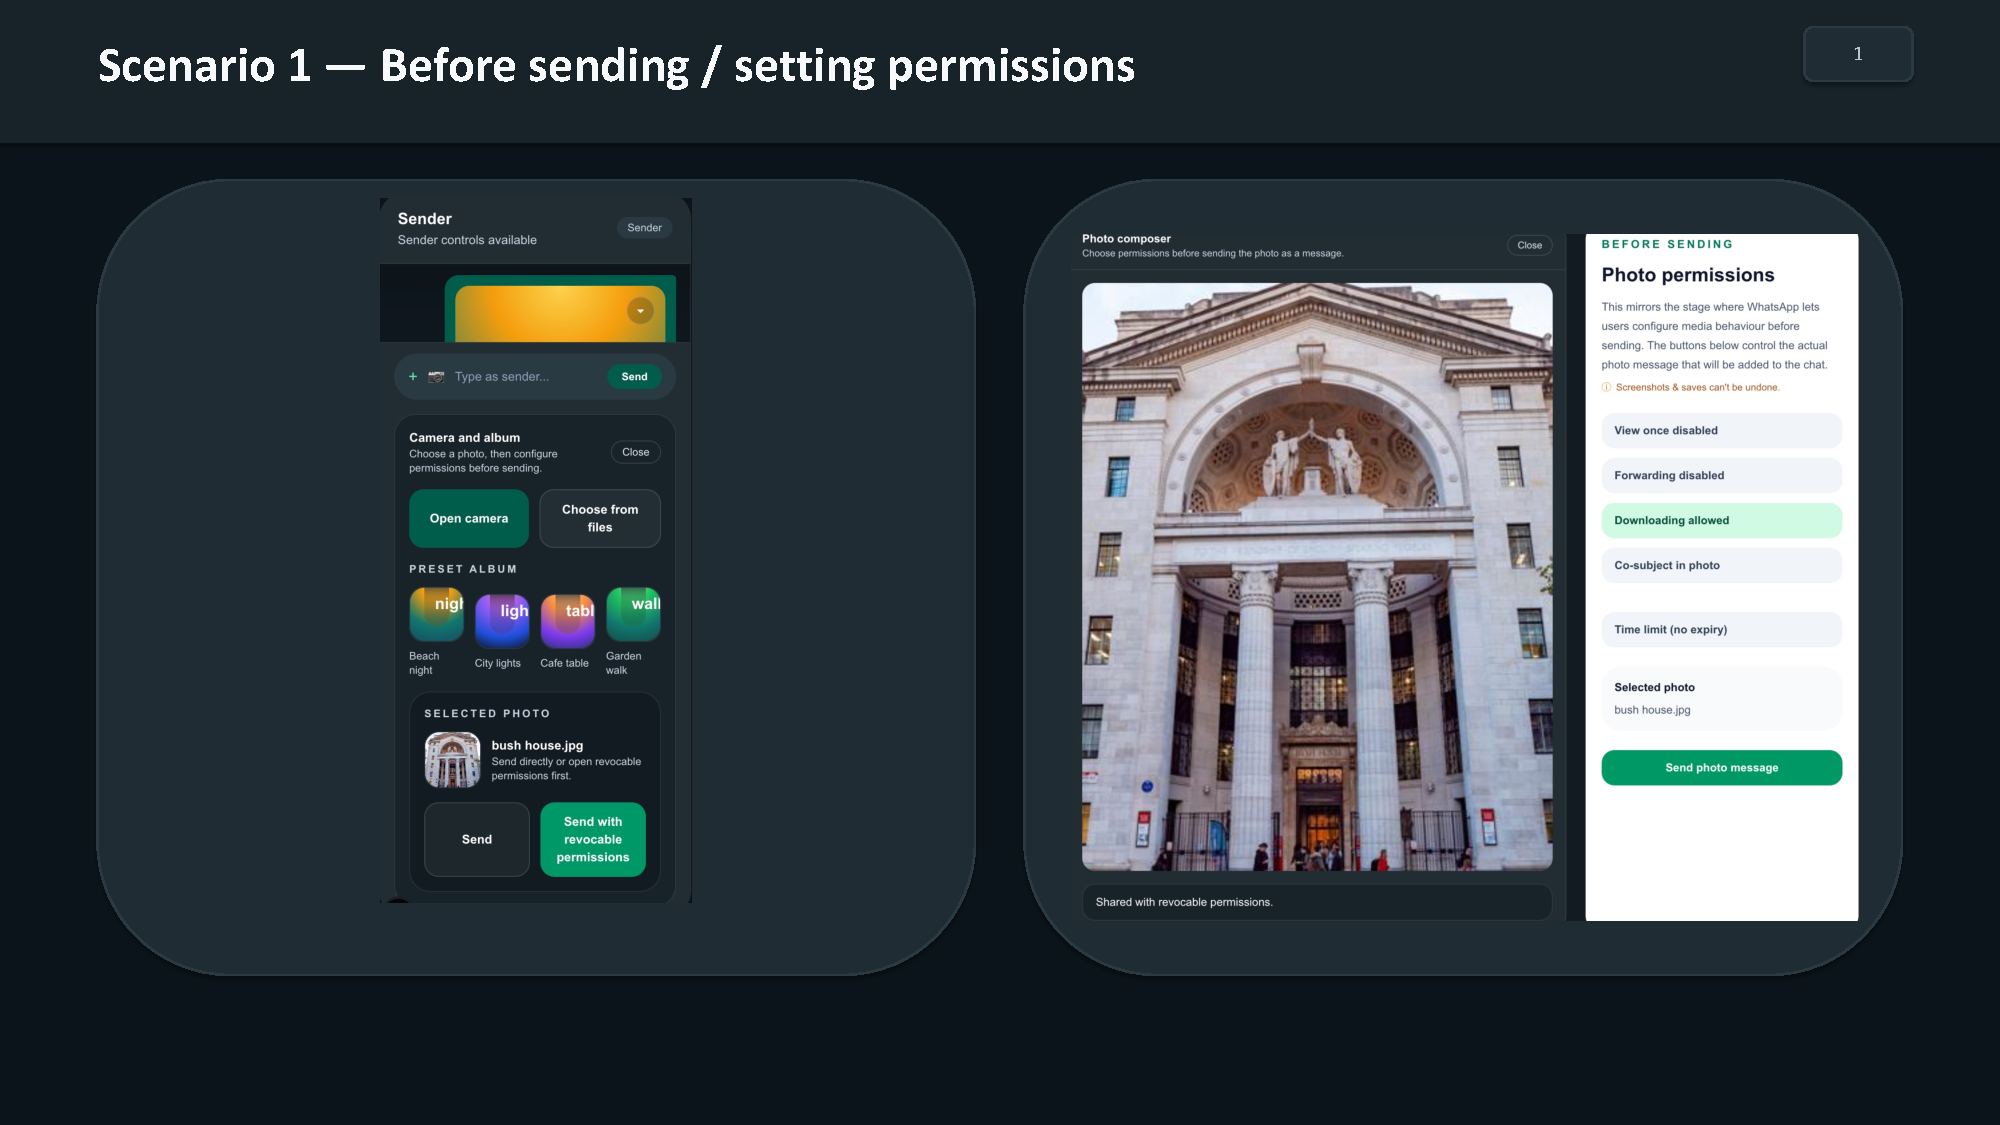
\includegraphics[page=1,width=\textwidth,height=0.88\textheight,keepaspectratio]{appendix-materials/interview/interview-scenario-slides.pdf}
\end{center}

\begin{center}
  \includegraphics[page=2,width=\textwidth,height=0.88\textheight,keepaspectratio]{appendix-materials/interview/interview-scenario-slides.pdf}
\end{center}
\newpage
\begin{center}
  \includegraphics[page=3,width=\textwidth,height=0.88\textheight,keepaspectratio]{appendix-materials/interview/interview-scenario-slides.pdf}
\end{center}

\begin{center}
  \includegraphics[page=4,width=\textwidth,height=0.88\textheight,keepaspectratio]{appendix-materials/interview/interview-scenario-slides.pdf}
\end{center}
\newpage
\begin{center}
  \includegraphics[page=5,width=\textwidth,height=0.88\textheight,keepaspectratio]{appendix-materials/interview/interview-scenario-slides.pdf}
\end{center}

